\section{Resultados}
En la presente sección se presentarán los resultados de la ejecución de los experimentos planteados. Se presentarán los resultados de forma gráfica para cada uno de los casos a evaluar. Cabe aclarar que aunque se hicieron 10 repeticiones para ambos algoritmos, en esta seción de resultados solamente se va a presentar el promedio de las 10 repeticiones, debido a que el objetivo es mostrar la complejidad temporal promedio. \\


\subsection{Gráficas de resultados}
En la siguiente sección se procesarán los resultados obtenidos anteriormente mediante un programa de python que utiliza la librería Matplotlib para representar los resultados de una manera gráfica. Se mostrará una gráfica logarítmica para cada uno de los algoritmos que mostrará el orden de la complejidad temporal de estos para entradas de distintos tamaños. A continuación en la figura 3 se muestra la gráfica para el algoritmo de fuerza bruta.\\
\begin{figure}[!htbp]
    \centering
    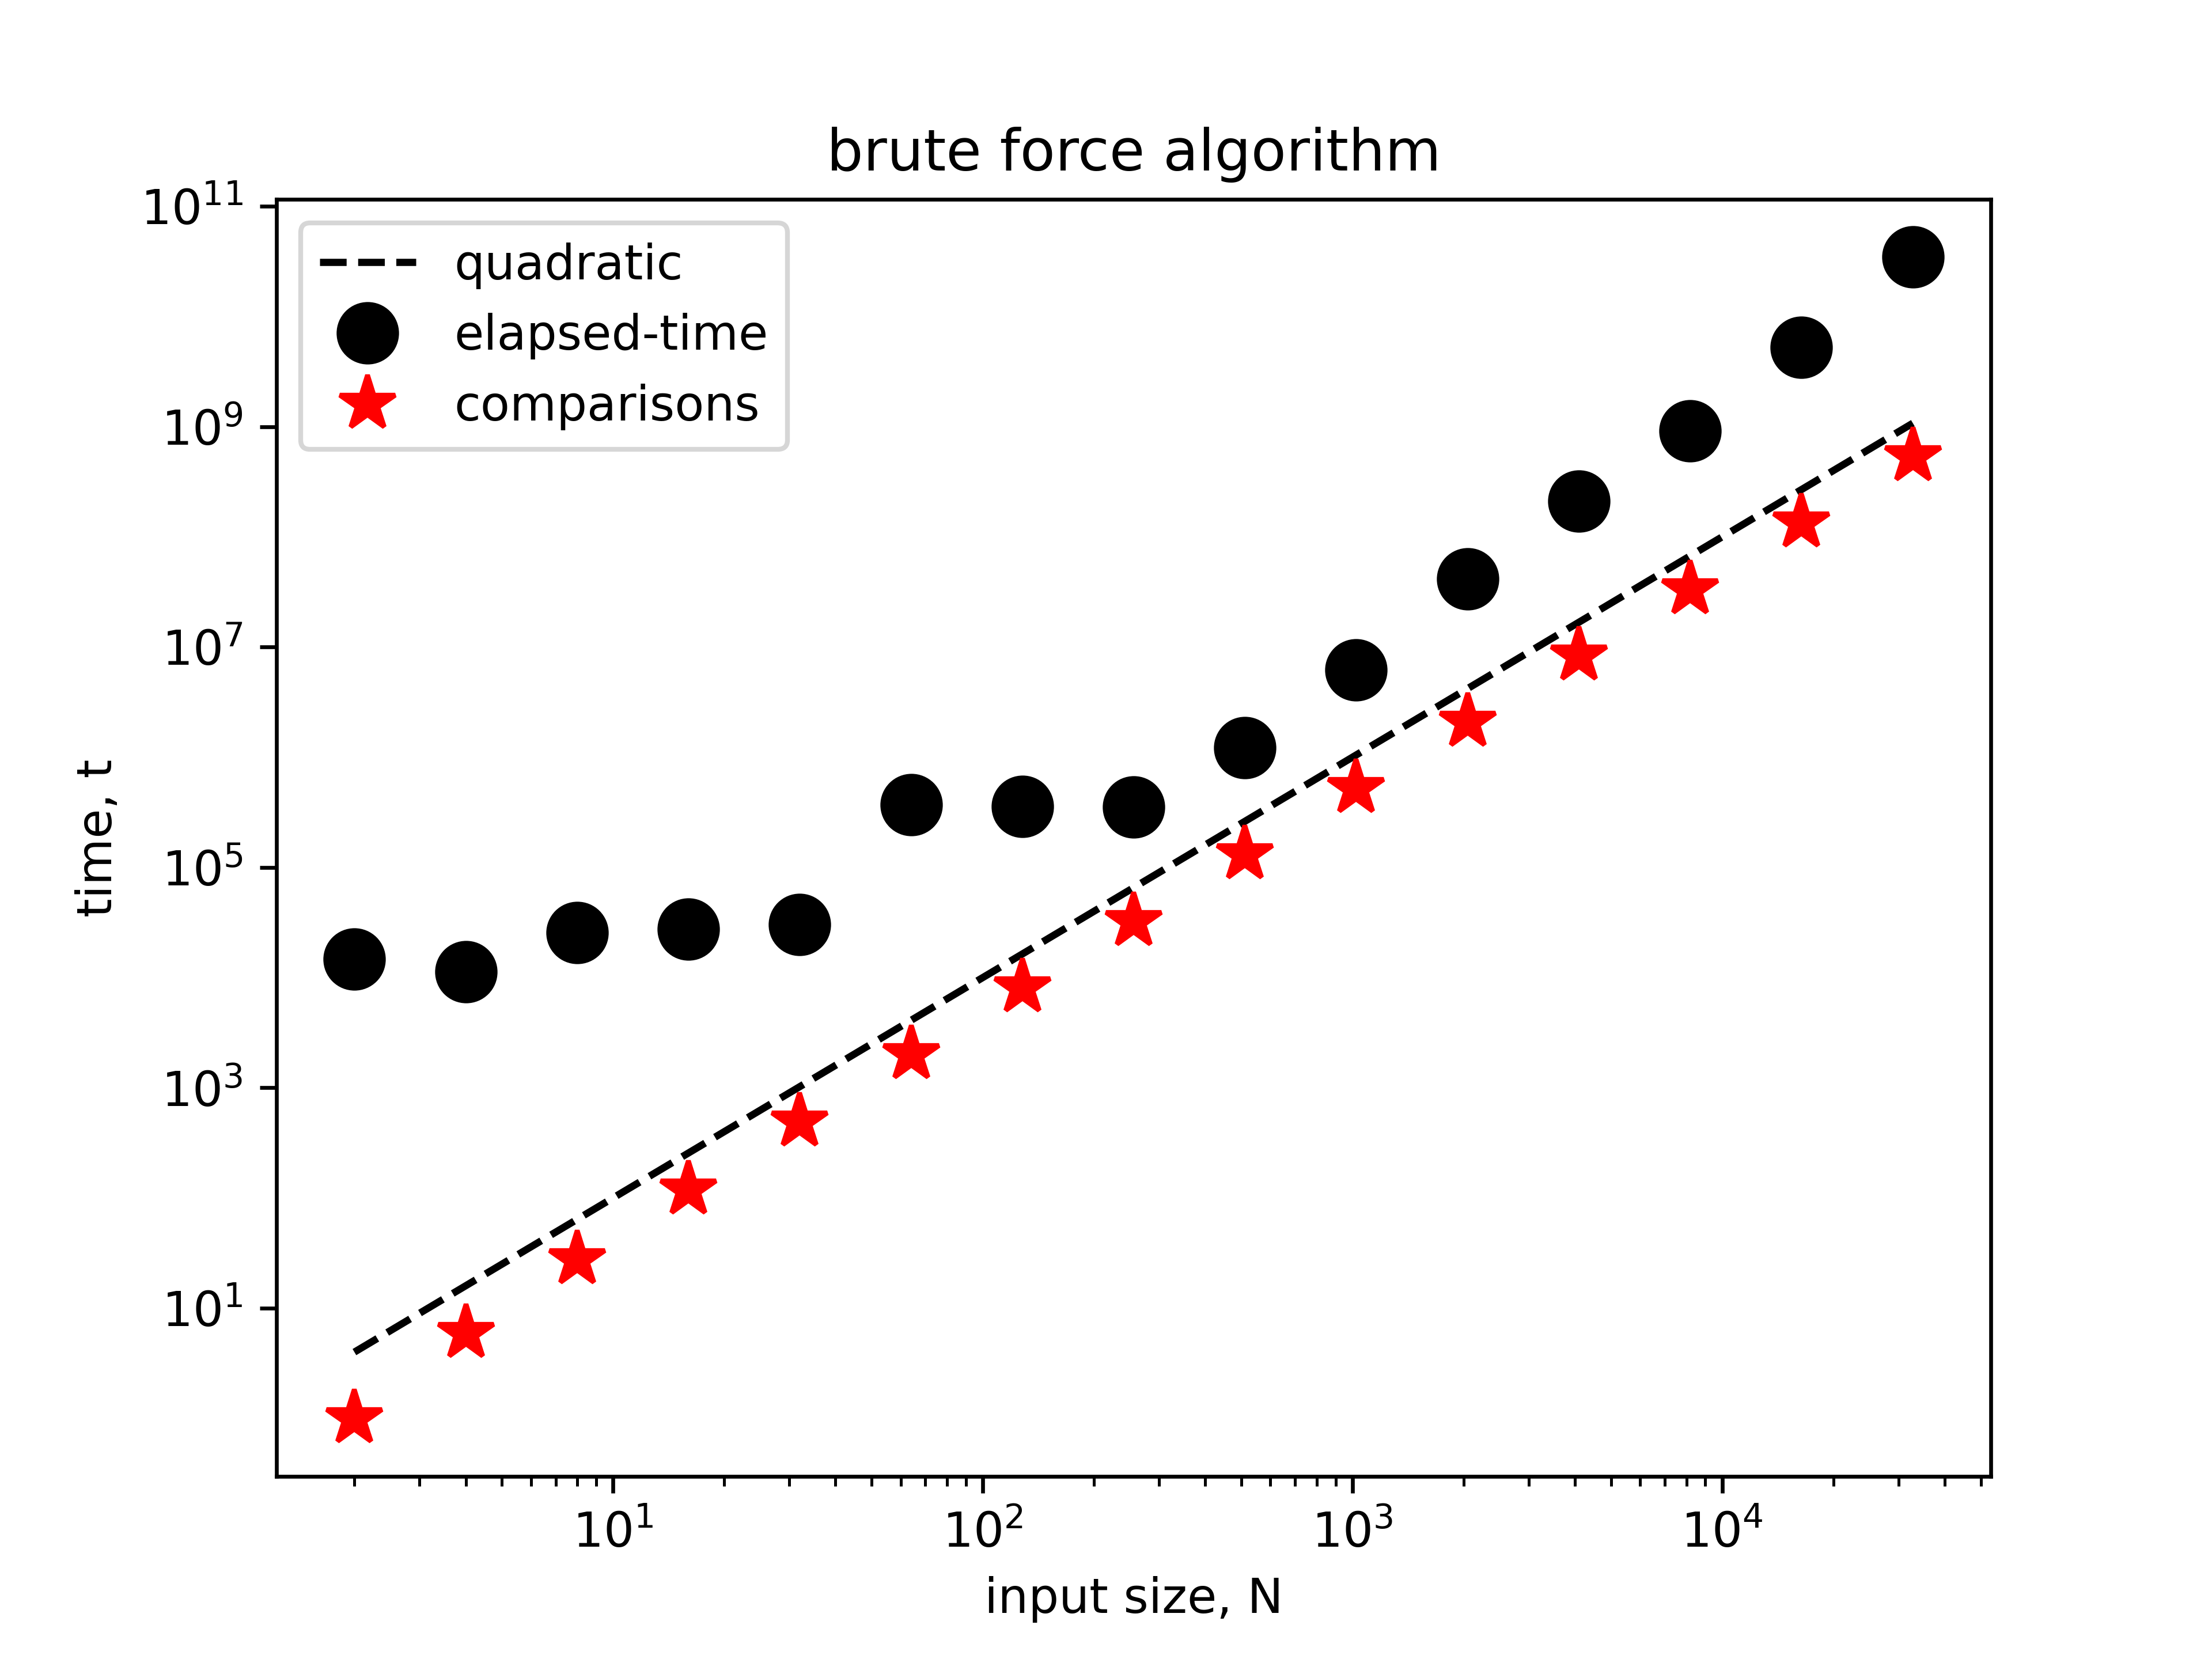
\includegraphics[width=.7\textwidth,height=.5\textwidth]{figures/brute force.png}
    \caption{Gráfica complejidad temporal algoritmo de fuerza bruta}
    \label{fig:my_label}
\end{figure}
La siguiente gráfica es la del algoritmo recursivo. Se puede ver esta en la figura 4.\\
\begin{figure}[!htbp]
    \centering
    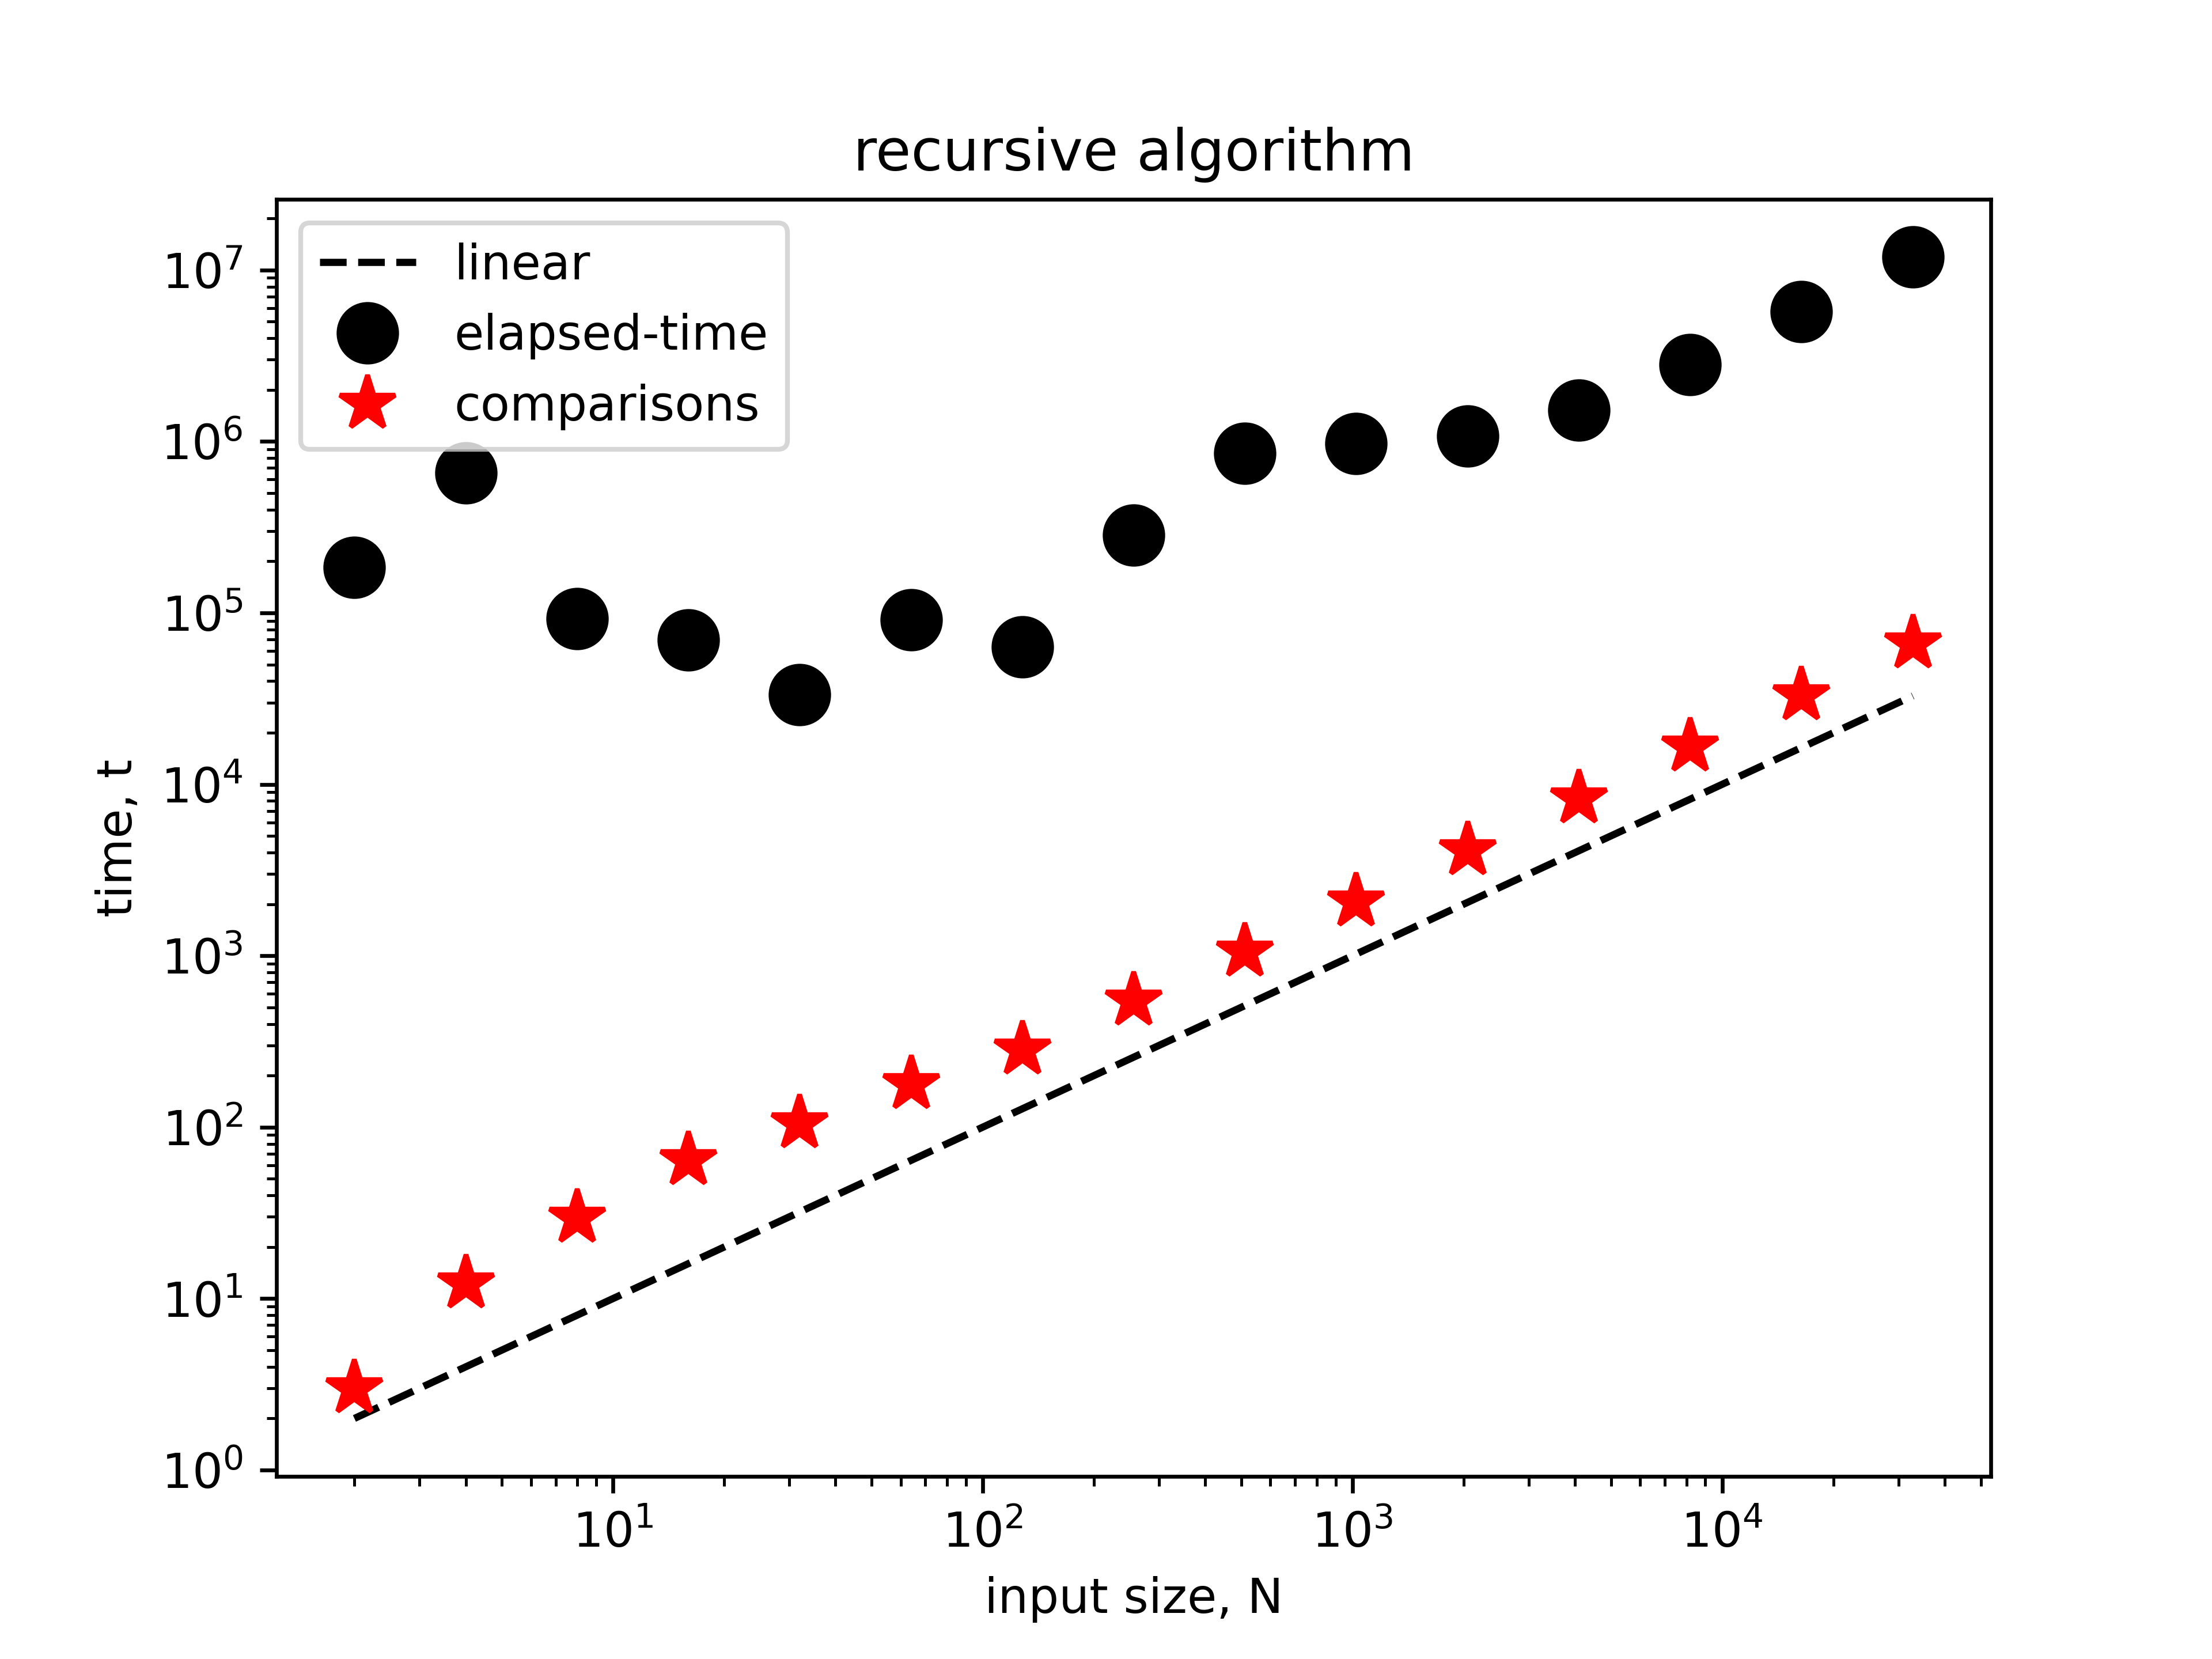
\includegraphics[width=.7\textwidth,height=.5\textwidth]{figures/recursive.png}
    \caption{Gráfica complejidad temporal algoritmo recursivo}
    \label{fig:my_label}
\end{figure}